\documentclass[a4paper]{article}

%% Language and font encodings
\usepackage[english]{babel}
\usepackage[utf8x]{inputenc}
\usepackage[T1]{fontenc}

%% Sets page size and margins
\usepackage[a4paper,top=3cm,bottom=2cm,left=3cm,right=3cm,marginparwidth=1.75cm]{geometry}

%% Useful packages
\usepackage{amsthm}
\usepackage{amsmath}
\usepackage{amssymb}
\usepackage{comment}
\usepackage{graphicx}
\usepackage[colorinlistoftodos]{todonotes}
\usepackage[colorlinks=true, allcolors=blue]{hyperref}
\usepackage{mathabx}
\usepackage{tikz}

\setlength\parindent{0pt}

\title{CS 4780/5780 Homework 5\vspace{-10pt}}
% \author{Due: Tuesday 04/10/18 11:55pm on Gradescope}
\date{\vspace{-0pt}}

\begin{document}
\maketitle

\subsection*{Problem 1: Derivation for Hard-margin Linear SVMs}
\textbf{a)} 

The hard-margin linear SVM solution gives the "best" separating hyperplane, i.e. the one that maximizes the margin to the nearest data points, whereas the perceptron gives any seperating hyperplane.

\begin{comment}
\textbf{b)}

$\min_{w,b}\frac{1}{\lVert w \rVert_2} \min_{x_i \in D} |w^Tx_i + b|$ [Maximize the margin of the hyperplane]\\
s.t. $\forall i, y_i(w^Tx_i + b) \geq 0$ [Every training point is classified correctly]\\

\textbf{c)} 

$\min_i\|\mathbf{w}^\top\mathbf{x}_i+b\|=1 \implies \lVert \mathbf{w} \rVert_2\Bigg(\min_i\dfrac{\|\mathbf{w}^\top\mathbf{x}_i+b\|}{\lVert \mathbf{w} \rVert_2}\Bigg)=1 \implies \lVert \mathbf{w} \rVert_2(margin)=1 \implies \boxed{\lVert \mathbf{w} \rVert_2 = \frac{1}{\gamma}}$


\textbf{b)} 

In the optimal solution, all the points are classified correctly and these constraints are satisfied. Since $y_i \in \{-1,+1\}$, and $|w^Tx_i+b| \geq 1$ for all data points $x_i$, we can multiply $|y_i|$ by $|w^Tx_i+b|$ to get the single constraint $|y_i(w^Tx_i+b)| \geq 1$. However, using the fact that $\forall_i \ y_{i}(\mathbf{w}^T \mathbf{x}_{i}+b) \geq 1$, we can remove the absolute value and get $y_i(w^Tx_i+b) \geq 1$.\\
\end{comment}
\textbf{b)}
This is to prove the constraints are equivalent in the two formulations.\\
i. As in formulation A, $y_{i}$ and $(w^Tx_i+b)$ should have the same sign because their product is greater than $0$. Since $y_i \in \{-1,+1\}$, so $y_{i}(w^Tx_i+b)$ should have been larger or equal to $1$. Therefore, an optimal solution of A is a feasible solution in B.

ii. %In formulation B, $y_{i}(w^Tx_i+b)\geq 1$ could satisfy $y_{i}(w^Tx_i+b)\geq 0$. Since $y_i \in \{-1,+1\}$, so there must be one value that satisfies $ \left| \mathbf{w}^T \mathbf{x}_{i}+b \right | =1$.
To show that the solution is feasible with respect to A we must show that an optimal solution of B satisfies both constraints of A. To start, if $y_{i}(\mathbf{w}^T\mathbf{x}_i+b)\geq 1$ then $y_{i}(\mathbf{w}^T\mathbf{x}_i+b)\geq 0$ is satisfied. For the second constraint we know that since $y_i \in \{-1,+1\}$, then for all $\mathbf{x}_i$, $ \left| \mathbf{w}^T \mathbf{x}_{i}+b \right | \geq 1$. Now we must show that there exists an x that gives us exact equality($ \left| \mathbf{w}^T \mathbf{x}_{i}+b \right | = 1$). For contradiction let us suppose no such x exists. Then there is some $x^*$ such that $ \left| \mathbf{w}^T \mathbf{x^*}_{i}+b \right |$ is minimized and $ \left| \mathbf{w}^T \mathbf{x^*}_{i}+b \right | = c $ for some $c > 1$. Note that c must be greater than 1 because of the statement we showed earlier that for all $\mathbf{x}_i$, $ \left| \mathbf{w}^T \mathbf{x}_{i}+b \right | \geq 1$. But now we can divide $\mathbf{w}$ and $b$ by $c$ so that $ \left| \mathbf{w}^T \mathbf{x^*}_{i}+b \right | = 1$ and our objective function will decrease by a factor of $1/c^2$ which means that our solution was not optimal so we’ve gotten a contradiction. Therefore if the solution to B is optimal then some x must exist such that $ \left| \mathbf{w}^T \mathbf{x^*}_{i}+b \right | = 1$. Therefore, an optimal solution of B is a feasible solution for A.


iii. Both formulations have the same objective function and because we have justified above that any optimal solution for one is a feasible solution for the other. So their solutions must have the same optimal value. Otherwise, if one of them has a solution with low objective value, you use that point for the other problem and would obtain the same low object value. Therefore we show that an optimal solution for A is an optimal solution for B, and vice versa.

%In the optimal solution, all the points are classified correctly and these constraints are satisfied. Since $y_i \in \{-1,+1\}$, and $|w^Tx_i+b| \geq 1$ for all data points $x_i$, we can multiply $|y_i|$ by $|w^Tx_i+b|$ to get the single constraint $|y_i(w^Tx_i+b)| \geq 1$. However, using the fact that $\forall_i \ y_{i}(\mathbf{w}^T \mathbf{x}_{i}+b) \geq 1$, we can remove the absolute value and get $y_i(w^Tx_i+b) \geq 1$.\\ 

 
\subsection*{Problem 2: Hard- vs. Soft-margin SVMs}
\textbf{a)} 

The hard-margin SVM does not converge on non-linearly separable data but the soft-margin SVM does because the soft constraints introduce a slack variable which allows the initial constraints presented in the hard-margin version to be violated such that the optimization problem becomes solvable. \\
\begin{comment}
	content...

\textbf{b)} 

As $C\rightarrow\infty$, the soft-margin SVM becomes more similar to the hard margin SVM. As $C\rightarrow0^+$, the soft-margin SVM completely ignores the data. This is because $C$ represents the penalty for misclassifying a training point. \\

\textbf{c)} 

One way would be to split the training set into a validation set in order to compare different values for $C$. This could involve applying a telescopic search on $C$ values which will be covered in more detail in a later lecture. Of course, all of these decisions would depend on your confidence in the regularization within the context of the problem. In general, more noisy data will require more slack than a less noisy data set.\\
\end{comment}
%\subsection*{Problem 3: Thinking in Terms of the "margin"}
\textbf{b)} 
\[
\min_{x \in D} |\mathbf{\hat w}^\top\mathbf{x} + \hat b| = 1 \\
\implies \exists x \text{ s.t. } \mathbf{\hat w}^\top\mathbf{x} + \hat b = 1 \text{ OR } \mathbf{\hat w}^\top\mathbf{x} + \hat b = -1
\] \\

This only shows that at least on training datapoint lies on at least one of the two margin hyperplanes. \\

Now, let us proceed with the assumption that there is no point on one of the two margin hyperplanes. If this was the case, then the solution to the maximum margin optimization would yield different margin hyperplanes. This contradicts the given margin hyperplanes in the problem and so there must be at least one training datapoint on \textbf{each} hyperplane. \\

\begin{comment}
\textbf{b)} 
The constraint that $\min_{x \in D} |\mathbf{\hat w}^\top\mathbf{x} + \hat b| = 1$ is no longer satisfied and the margin has decreased. \\

\textbf{c)}
\begin{center}
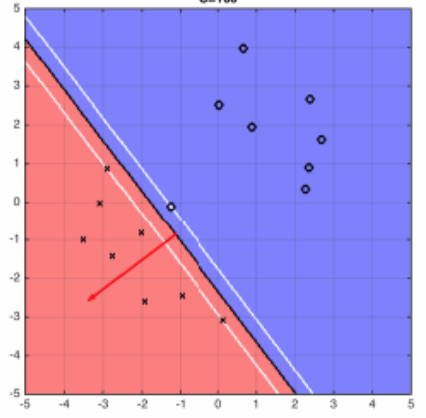
\includegraphics{SVM.png}
\end{center}
In your friend's scaled version, the margins would be moved further from the hyperplane, leaving at least two datapoints in between the margins.\\



\subsection*{Problem 4: MLE in terms of ERM}

\textbf{a)} 

\begin{align*}
    \hat{g} &= \arg\min_g \mathbb{E}_{(x,y)\sim\pi}\left[\log\frac{\pi(x,y)}{g(x,y)}\right] \\
    &= \arg\min_g \mathbb{E}_{(x,y)\sim\pi}\left[\log\pi(x,y) - \log g(x,y)\right] \\
    &= \arg\min_g \mathbb{E}_{(x,y)\sim\pi}\left[- \log g(x,y)\right] \\
\end{align*}

Thus, 
$$h(x) = g(x,*)$$
which uses currying and $h(x)$ is a function of $y$. It outputs a probability disribution, not a point estimation. 

Then the loss function is (cross-entropy loss): 
$$l = -\log (g(x,y)) = -\log( h(x)(y))$$

\textbf{b)} 

$$\hat{g} = \text{arg min}_g \sum_{(x,y)\in D} -\log(g(x,y))$$

\textbf{c)} 

\begin{align*}
   \hat{g} 
   &= \arg\min_g \sum_{(x,y)\in D} -\log(g(x,y))\\
   &= \arg\max_g\sum_{(x,y)\in D} \log(g(x,y))\\
   &= \arg \max_g \prod_{(x,y)\in D} g(x,y)
\end{align*}
\end{comment}

\end{document}
